\beginsong{Eine Hand voll Erde}[wuw={R. Bacher, D. Jocher}, pfii={125}, gruen={51}, index={Mit der Erde kannst du spielen}]

\beginverse
\endverse
\centering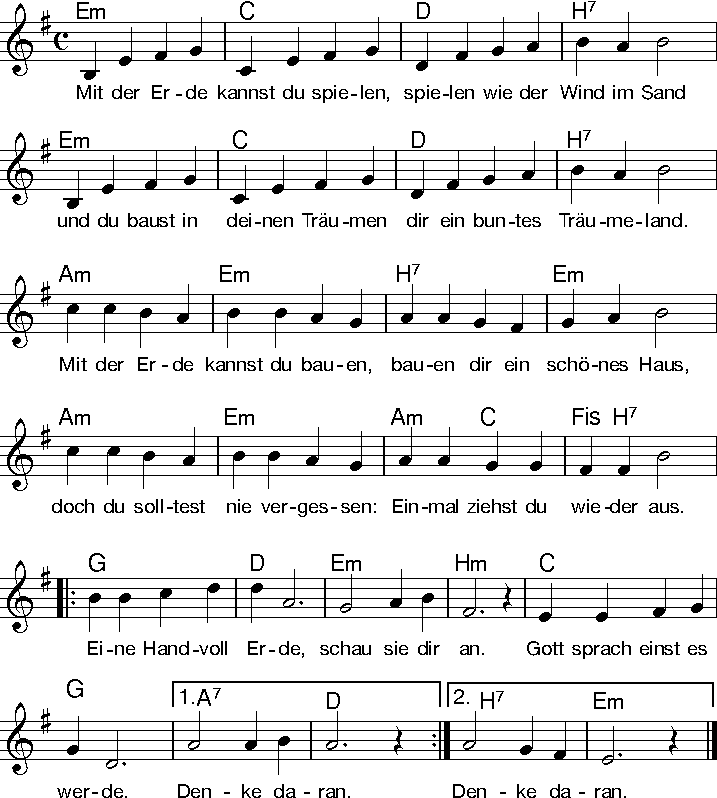
\includegraphics[width=1\textwidth]{Noten/Lied108.pdf}

\beginverse
\[Em]Auf der Erde \[C]kannst Du stehen,
\[C]stehen, weil der \[G]Grund dich \[H7]hält
\[Em]und so bietet \[C]Dir die Erde.
\[D]Einen Standpunkt \[G]in der \[H7]Welt
\[Am]in die Erde \[Em]kannst Du pflanzen
\[H7]Pflanzen einen \[Em]Hoffnungsbaum
\[Am]und er schenkt Dir \[Em]viele Jahre
\[Am]einen \[C]bunten \[F#]Blüten\[H7]traum.
\endverse

\beginchorus
\lrep \[G]Eine Hand voll \[D]Erde, \[Em]schau sie dir \[H7]an.
\[C]Gott sprach einst: Es \[G]werde! \[D]Denk \[G]daran! \rrep
\endchorus

\beginverse
^Auf der Erde ^darfst du leben,
^leben ganz und ^jetzt und ^hier
^und Du kannst das ^Leben lieben,
^denn der Schöpfer ^schenkt es ^dir.
^Uns're Erde ^zu bewahren
^zu bewahren ^das, was lebt,
^hat Gott Dir und ^mir geboten,
^weil er ^seine ^Erde ^liebt.
\endverse

\endsong
